\documentclass[11pt,a4paper]{article}
\usepackage[utf8]{inputenc}
\usepackage[T1]{fontenc}
\usepackage{amsmath}
\usepackage{amsfonts}
\usepackage{amssymb}
\usepackage{graphicx}
\usepackage{setspace}
\usepackage[left=2.5cm,right=2.5cm,top=2.5cm,bottom=2.5cm]{geometry}
\usepackage{float}
\usepackage[font=small,labelfont=bf]{caption}
\linespread{1.5}
\graphicspath{{./images}}

\setlength{\abovecaptionskip}{5pt}
\setlength{\belowcaptionskip}{0pt}

\begin{document}

\begin{center}
    \normalsize{Application for Admission to the PHD Programme in the Faculties of Engineering}\\
    \textbf{\Large{A Control Framework for Electroadhesive Perching and Sustained Hanging of UAVs using Electrorheological Fluids}}\\
    \normalsize{Zilin Chen}
\end{center}

\section{Background}
\subsection{Literature Review}
Data shows that in 2022, the market size of the global drone industry is over \$30 billion, and it is expected to expand to \$55 billion in 2030~\cite{nonami2025overview}. People use UAVs in all kinds of areas, including remote sensing, photogrammetry, package-delivering etc.~\cite{COLOMINA201479} Drones have great flexibility and can reach locations that are not restricted by terrain. At the same time, compared to ground mobile robots, drones usually have higher moving speed.\\
However, drones are also subject to certain limitations. Their \textbf{flight endurance} is considerably shorter than that of ground-based mobile robots, typically lasting only a few hours—often less than one hour~\cite{kim2018drone}. Despite various attempts to extend drone flight time, the energy density of existing storage materials remains a fundamental constraint, resulting in still limited operational duration. It is noted that in many applications, drones are only required to hover at designated locations to perform tasks. Yet, hovering itself consumes a significant amount of energy, which largely constitutes wasted power since no useful locomotion is involved.\\
To substantially extend the drone’s operational endurance, we propose a perching mechanism that allows the drone to attach to static structures, enabling complete shutdown of the rotors and eliminating the high energy consumption associated with stationary hovering. A key enabler of this approach is the use of \textbf{electrorheological fluid (ERF)}, a smart material whose rapid and reversible adhesion properties make it ideally suited for this application. In contrast to other compliant gripping technologies—such as the positive-pressure layer jamming (PPLJ) developed by Professor Haijun Su’s team~\cite{crowley20223d} or conventional dielectric elastomer actuators (DEAs)—ERF exhibits superior performance in conforming to and adhering on relatively flat surfaces~\cite{o2008review}.\\
Electrorheological fluids belong to a class of smart materials that undergo a reversible, electric-field-induced transition in rheological state. Typically consisting of dielectric particles dispersed in an insulating fluid, ERFs demonstrate a dramatic increase in viscosity under an applied electric field. When exposed to a sufficiently strong field, the particles polarize and rapidly form chain- or column-like microstructures aligned with the field direction. This transition leads to a near-instantaneous change from liquid-like to solid-like behavior, known as the electrorheological (ER) effect~\cite{liu2012electrorheological}.\\
In the context of drone perching, ERF is integrated into the contact mechanism. Applying voltage induces solidification of the fluid, creating strong and controllable adhesion almost instantaneously. This allows the drone to perch securely on surfaces at various orientations—vertical, inverted, or inclined. When the voltage is removed, the ERF reverts to its liquid state, adhesion ceases, and detachment occurs with minimal energy cost~\cite{kuznetsov2022electrorheological}. This fast, reversible, and electrically switchable adhesion offers a robust technological foundation for energy-efficient perching in complex environments.\\
Further advancing this concept, Professor Huichan Zhao and her team developed a novel variant of ERF named \textit{VSERF} (voltage-switchable electrorheological fluid)~\cite{pan2022stretchable}. This material demonstrates remarkable persistence in adhesion, capable of sustaining attachment for over 25 minutes per activation and accumulating more than 64 hours of total operation. Such performance provides a practical material solution for long-duration drone perching, significantly extending mission time without consuming propulsion energy.
\vspace{10pt}
\begin{figure}[H]
    \centering
    
\includegraphics[width = \textwidth]{key_tech.png}
    \caption{\textbf{(a)}VSERF developed by Prof.\  Huichan Zhao and her team, can attach to different surfaces.~\cite{pan2022stretchable}\;\textbf{(b)}Demonstration for Betaflight-controller in a simulation environment.~\cite{mdss}\;\textbf{(c)}A lightweight small-scale object recognition system for drones, developed by Zhengxin Zhang based on YOLOv8~\cite{zhang2023drone}\;\textbf{(d)}System Architecture of the Drone Platform}
\end{figure}
\newpage
\noindent
In addition to the grasping mechanism, the integration of a \textbf{flight controller} and a \textbf{visual recognition system} is essential to enable the drone to autonomously identify and approach suitable perching locations.\\
Numerous open-source flight controllers are available for quadrotor UAVs. Among these, an open-source flight controller named \textbf{\textit{Betaflight}}~\cite{betaflight} is particularly notable for its high performance and is widely adopted in autonomous drone racing applications~\cite{kaufmann2023champion}. It offers substantial flexibility and controllability, facilitating precise trajectory tracking and attitude stabilization, which allows the drone to reliably achieve desired positions and orientations~\cite{qin2024time}.\\
For \textbf{visual recognition}, existing systems such as YOLO and visual SLAM provide robust support for identifying perch-compatible objects. Professor Hongbin Ji and his team developed a feature pyramid network that enhances image resolution, improving the drone’s capability to detect small objects~\cite{chen2023high}. Similarly, Zhengxin Zhang introduced an improved YOLOv8-based algorithm that enhances detection performance for small, densely clustered targets~\cite{zhang2023drone}. These advances are crucial for enabling drones to locate typical perching structures such as streetlights and tree branches with high accuracy.
\subsection{Past Experience}
During my previous research, I gained hands-on experience working with the core codebase of \textbf{\textit{Betaflight}}, where I utilized its open-source platform to develop a simulator for angular velocity planning and implemented a demonstration for attitude control. I also addressed the yaw angle optimization planning problem, which has provided me with a solid background in optimization-based trajectory planning. Additionally, my practical experience with \textbf{Open-MV} and computer vision has equipped me with the skills necessary for real-time target detection.

\section{Methodology}
This research develops and validates a hierarchical control framework to enable fully autonomous UAV perching using VSERF\@. The methodology integrates four technical thrusts, progressing from modeling and simulation to physical validation, as shown in Figure~\ref{ORF}.
\begin{figure}[http]
    \centering
    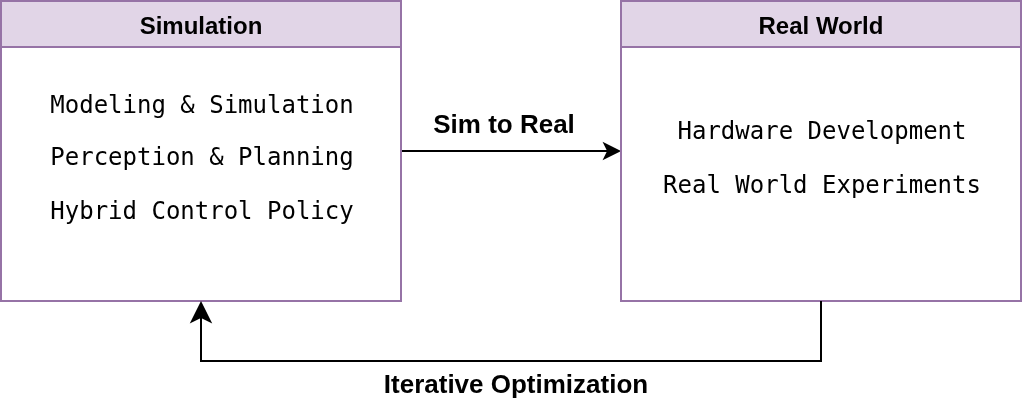
\includegraphics[width = 0.6\textwidth]{ORF.png}
    \caption{\textbf{Research Framework.} The project integrates theoretical modeling, simulation, learning-based policy training, and hardware experimentation in an iterative loop to ensure robustness and Sim-to-Real transfer.}\label{ORF}
\end{figure}

\subsection{High-Fidelity System Modeling and Simulation}
This phase creates a virtual testbed that accurately captures the dynamics of the UAV and the VSERF perching mechanism.


\subsubsection{UAV Dynamics Modeling}
We are going to derive a 6-degree-of-freedom (6-DOF) nonlinear dynamic model of the quadrotor, incorporating aerodynamic effects and motor dynamics. This model serves as the plant for controller design.

\subsubsection{VSERF Contact Dynamics Modeling}
A critical component is modeling the electroadhesive contact. We will establish a force model based on VSERF material properties, relating the applied electric field strength and contact area to the generated adhesive force and friction. This model will accounts for surface roughness and inclination.

\subsubsection{Simulation Environment Setup}
We will implement these models in \textbf{MuJoCo}~\cite{todorov2012mujoco}, a high-performance physics simulator well-suited for contact-intensive tasks. This simulator can simulate not only the various parameters of the flight process but also the unstable contact conditions during the adsorption process, making it ideal for this study.

\subsection{Integrated Perception and Planning}
This module enables the drone to autonomously identify perching sites and plan trajectories. We will deploy a lightweight convolutional neural network (CNN), based on an improved \textbf{YOLOv8} architecture~\cite{zhang2023drone}, for real-time object detection. The network identifies potential perching sites and assesses their suitability based on surface characteristics.\\
After target identification, a Perspective-n-Point (PnP) algorithm, fused with IMU data, estimates the relative 6D pose of the target. A sampling-based planner then generates a smooth, collision-free trajectory to a pre-contact pose near the surface.

\subsection{Hybrid Control Policy Development}
The core innovation addresses the seamless transition from free flight to adhered perching through a hybrid control architecture governed by a finite state machine (FSM).

\begin{figure}[H]
    \centering
    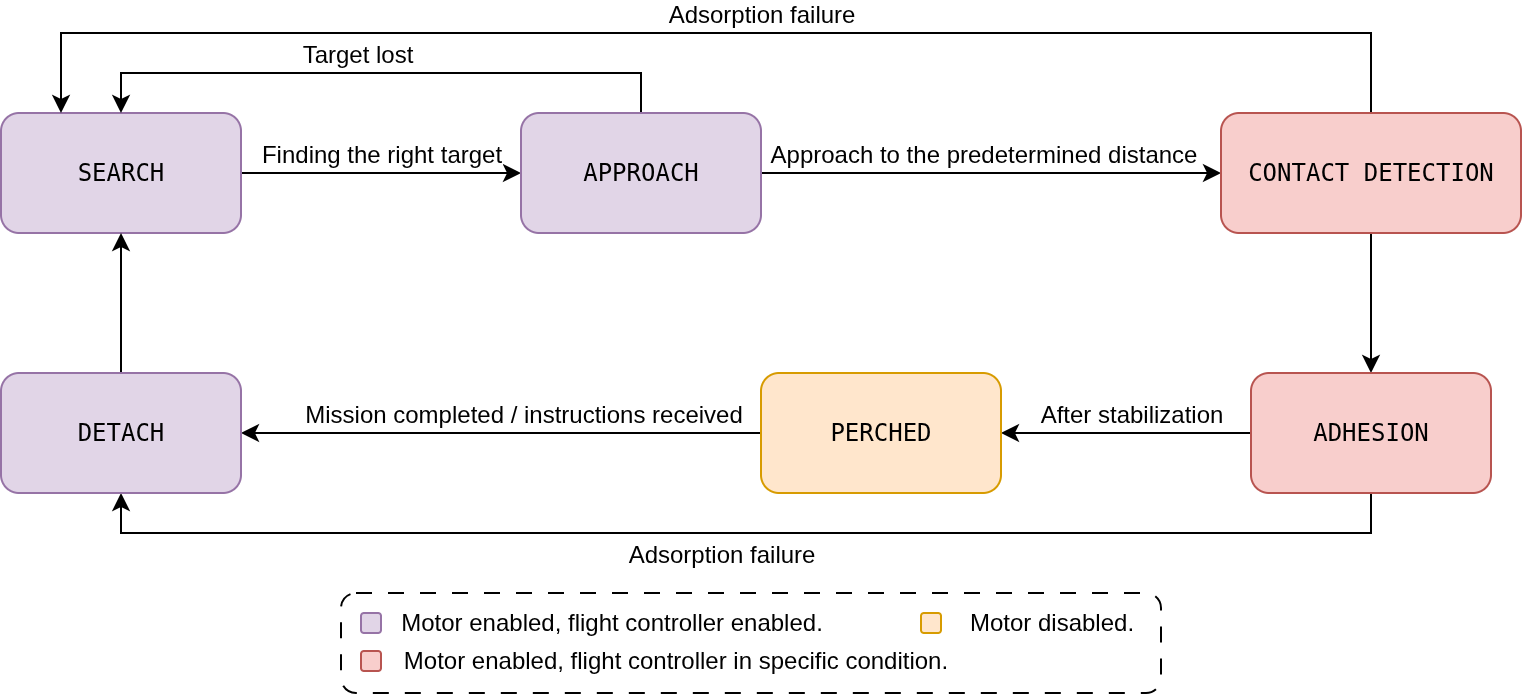
\includegraphics[width = \textwidth]{SM.png}
    \caption{\textbf{Hybrid Control State Machine.} The system transitions between discrete states based on sensor triggers, ensuring safe and precise mode switching during the perching maneuver.}\label{SM}
\end{figure}

\subsubsection{Model-Based Flight Controller}
For gross motion, a Nonlinear Model Predictive Control (NMPC) or a cascaded PID controller ensures stable trajectory tracking.

\subsubsection{Learning-Based Final Approach Policy}
The final approach and contact phase require delicate maneuvers. We train a \textbf{Deep Reinforcement Learning (DRL)} policy, using the Soft Actor-Critic (SAC) algorithm in simulation, to master this phase. The policy maps states to continuous drone commands, minimizing contact impulse and achieving perfect surface alignment.

\subsubsection{Mode Switching Logic}
A finite state machine (Figure~\ref{SM}) manages transitions between operational states. Key triggers include proximity to the target, contact detection via a touchdown sensor or IMU data, and successful adhesion confirmation.

\subsection{Hardware Integration and Experimental Validation}
We build a prototype to validate the simulation results in real-world conditions.

\subsubsection{Hardware Platform}
The hardware platform consists of:
\begin{itemize}
    \item A custom-built quadrotor with a \textbf{Betaflight} flight controller.
    \item A lightweight \textbf{VSERF perching module} with a high-voltage driver circuit.
\end{itemize}

\subsubsection{System Integration}
We establish a robust communication protocol (e.g., ROS 2) between the computing unit, flight controller, and the perching mechanism. A systematic experimental evaluation measures key performance metrics:
\begin{itemize}
    \item Perching Success Rate on different surfaces and angles.
    \item Energy Consumption compared to stationary hovering.
    \item Attachment/Detachment Time and long-term reliability.
\end{itemize}

\section{Timeline}
The research will last for a standard four-year PhD period, structured to progress systematically from theoretical development and simulation to system integration and experimental validation.

\begin{itemize}
\item \textbf{Year 1: Foundation and Modeling}
\begin{itemize}
\item \textit{Months 1--6}: Literature review on electrorheological fluids, UAV perching, and autonomous flight control.
\item \textit{Months 7--12}: Develop dynamic and kinematic models of the quadrotor and VSERF perching system. Begin physics-based simulations.
\end{itemize}

\item \textbf{Year 2: Control and Learning Policy Development}
\begin{itemize}
\item \textit{Months 13--18}: Design hybrid control framework and transition logic between flight and perching modes.
\item \textit{Months 19--24}: Train and validate RL policies in simulation for target identification and perching. Integrate visual recognition modules.
\end{itemize}

\item \textbf{Year 3: System Integration and Preliminary Testing}
\begin{itemize}
\item \textit{Months 25--30}: Build and integrate VSERF hardware with UAV platform. Calibrate sensors and actuators.
\item \textit{Months 31--36}: Conduct bench tests and controlled flight experiments. Evaluate adhesion and vision systems.
\end{itemize}

\item \textbf{Year 4: Validation and Thesis Completion}
\begin{itemize}
\item \textit{Months 37--42}: Perform real-world experiments across various surfaces and conditions.
\item \textit{Months 43--48}: Analyze data, optimize performance, and refine controls. Prepare publications and finalize thesis.
\end{itemize}
\end{itemize}

\section{Outcomes and Value}
This research aims to deliver both theoretical insights and practical technologies that advance the capabilities of unmanned aerial vehicles. The anticipated outcomes include:

\begin{itemize}
    \item A novel control framework integrating model-based and learning-based methods for robust and autonomous UAV perching.
    \item A hardware prototype demonstrating energy-efficient perching and sustained hanging using VSERF technology.
    \item High-fidelity simulation models and datasets that can be reused by the research community.
    \item Publications in top-tier robotics and smart materials conferences and journals.
\end{itemize}
\begin{figure}[H]
    \centering
    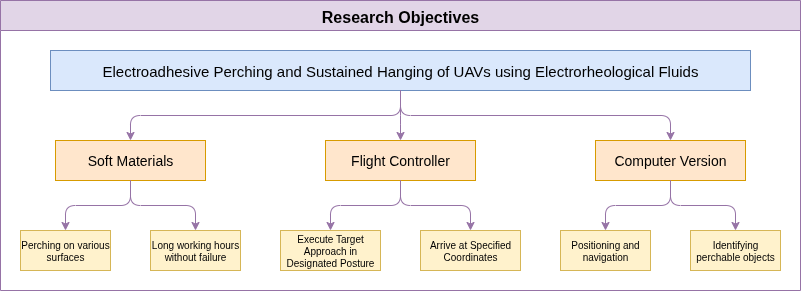
\includegraphics[width = \textwidth]{direction.png}
    \caption{Research Framework Diagram}
\end{figure}
\noindent
The successful implementation of this project will significantly extend UAV operational endurance in applications such as environmental monitoring, infrastructure inspection, and surveillance. By enabling drones to perch for long periods without consuming energy, this technology reduces operational costs and increases mission flexibility. Furthermore, the integration of smart materials like VSERF into robotic systems opens new pathways for future research in adaptive and energy-aware autonomous systems.\\
The primary challenge and innovative aspect of this project lies in the requirement that the drone must autonomously identify a suitable perching target and approach it in a specific spatial attitude. Unlike conventional flight controllers, which permit continuous obstacle avoidance even near the target, our approach necessitates a direct and precise trajectory alignment in the final approach phase. Moreover, the critical timing for activating the electroadhesive mechanism and disengaging the flight control system upon contact introduces a complex hybrid control challenge. The development of a robust control strategy capable of handling this transition seamlessly represents the core innovation of this work.

\vspace{150pt}
\bibliographystyle{IEEEtran}
\bibliography{references}

\end{document}